\documentclass[tikz, conver=pdf2svg,utf8]{standalone}
\usepackage{tikz}
\usepackage[AutoFakeBold=true,AutoFakeSlant=true]{xeCJK}
\usepackage[zihao=-4,UTF8,heading=true]{ctex}
\usepackage[simplified]{pgf-umlcd}
\usetikzlibrary{positioning} %不加方向运算可能出错
\usetikzlibrary{arrows.meta} %箭头

\setCJKmainfont{微软雅黑}
\begin{document}
	\thispagestyle{empty}
    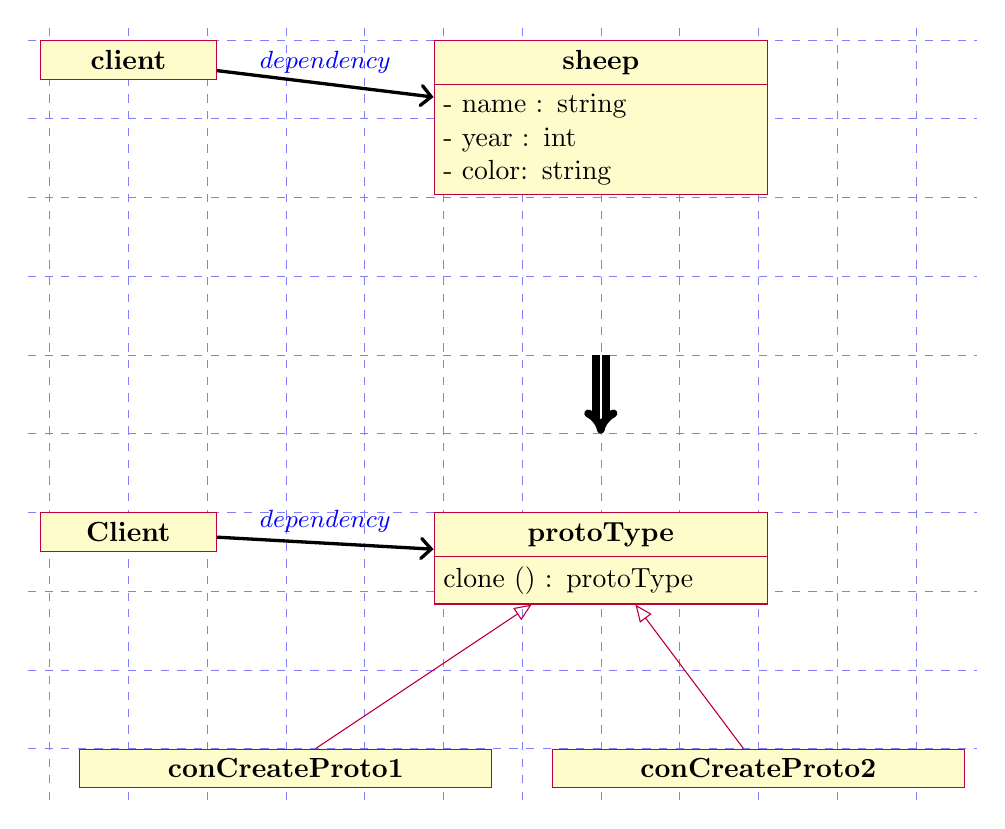
\begin{tikzpicture}[show background grid]
        \begin{class}[text width=4cm]{sheep}{0,0}
            \attribute{- name : string}
            \attribute{- year : int}
            \attribute{- color: string}
        \end{class}
        \begin{class}[text width=2cm]{client}{-6, 0}

        \end{class}
        \draw[umlcd style, black,->, very thick] (client) --
            node[anchor=south, blue]{\small $dependency$} (sheep);
        \draw[-Implies, double,line width=0.1cm] (0,-4) -- (0,-5);

        \begin{class}[text width=4cm]{protoType}{0,-6}
            \operation {clone () : protoType}
        \end{class}
        \begin{class}[text width=2cm]{Client}{-6,-6}

        \end{class}
        \draw[umlcd style, black,->, very thick] (Client) --
                node[anchor=south, blue]{\small $dependency$} 
                (protoType);
        \begin{class}{conCreateProto1}{-4, -9}
            \inherit{protoType}
        \end{class}
        \begin{class}{conCreateProto2}{2, -9}
            \inherit{protoType}
        \end{class}
    \end{tikzpicture}
\end{document}